\documentclass{beamer}
\mode<presentation>
\usetheme{CambridgeUS}
\usepackage[russian]{babel}
\usepackage[utf8]{inputenc}
\usepackage[T2A]{fontenc}
\usepackage{sansmathaccent}

\usepackage{verbatim}
\usepackage{alltt}

\pdfmapfile{+sansmathaccent.map}
\title[Software Design]{Класс как основной механизм абстракции}
\author{Наумов Д.А., доц. каф. КТ}
\date[30.09.2019] {Основы программной инженерии, 2019}

\begin{document}

%ТИТУЛЬНЫЙ СЛАЙД
\begin{frame}
  \titlepage
\end{frame}
  
%СОДЕРЖАНИЕ ЛЕКЦИИ
\begin{frame}
  \frametitle{Содержание лекции}
  \tableofcontents  
\end{frame}
  
\section{Структура и организация определения класса}
\begin{frame}
\textbf{Задача классов} - предоставить программисту инструмент для создания новых типов данных с тем, чтобы их можно было без ограничений использовать в программе наряду со встроенными типами.

\textbf{Тип данных} является вопложением некоторой концепции (пример: целые числа), которое определяется рядом характеристик:
\begin{itemize}
\item областью применения типа;
\item способом представления типа в памяти;
\item множеством операций, разрешенных для этого типа;
\item множеством совместимых типов.
\end{itemize}
Новые типы создаются для воплощения концепций, которые \textit{не выражаются непосредственно} (или адекватно) встроенными типами.
\end{frame}

\subsection{Элементы-данные и элементы-действия}
\begin{frame}
\begin{itemize}
\item \textbf{Класс} - элемент абстракции.
\item Определяя класс, мы создаем программную сущность, позволяющую выделить существенные характеристики некоторого объекта, отличающие его от других видов объектов.
\item Мы отделяем друг от друга элементы объекта, определяющие его устройство (\textbf{элементы-данные}), от элементов, определяющих его поведение (\textbf{элементы-действия}).
\item Данные, объявленные внутри определения класса, могут, в частности, быть п\textbf{еременными-членами класса} и \textbf{константами-членами класса}. 
\item Функции, объявленные внутри определения класса, называются \textbf{функциями-членами класса}, или \textbf{методами} класса.
\end{itemize}
\end{frame}

\begin{frame}[fragile]{Пример. Очередь}
\begin{alltt}
1 type
2   QueueInt = class(TObject) 
3     public
        //массив для хранения данных
4       body: array[0..MAXSIZE] of integer; 
5       size: integer;   //Предельный размер 
6       length: integer; //Текущая длина очереди
7       last: integer;   //Индекс последнего 
                         //занесенного элемента
8       next: integer;   //Индекс извлекаемого 
                         //Элемента очереди                      
9       procedure Init(CustomSize: integer); //Инициализация   
10      procedure Enqueue(Elem: integer); //Записать элемент
11      function Dequeue(): integer; //Извлечь элемент
12      procedure Print; //Печать содержимого
13 end;
\end{alltt}
\end{frame}

\subsection{Управление доступом к членам класса}
\begin{frame}
\textbf{Разграничение доступа} к членам класса преследует две основные цели:
\begin{itemize}
\item обеспечение связывания функций-членов класса с переменными-членами
класса таким образом, чтобы только эти функции непосредственно зависели от представления класса и имели непосредственный доступ к объектам класса;
\item обеспечение инкапсуляции, т. е. отделения внешнего интерфейса класса от его реализации.
\end{itemize}

Спецификаторы доступа:
\begin{itemize}
\item спецификатор \textbf{private} - закрытые члены класса, могут использоваться только методами класса;
\item спецификатор \textbf{public} - открытый интерфейс класса, разрешен доступ не только функциям-членам класса, но и обращение из-за пределов объявления класса;
\item \textbf{protected} - будет рассмотрен позже;
\item \textbf{published} - будет рассмотрен позже.
\end{itemize}
\end{frame}

\begin{frame}[fragile]{Пример. Инкапсуляция}
\begin{alltt}
1 type
2   QueueInt = class(TObject) 
3     private
        //массив для хранения данных
4       body: array[0..MAXSIZE] of integer; 
5       size: integer;   //Предельный размер 
6       length: integer; //Текущая длина очереди
7       last: integer;   //Индекесы первого и                          
8       next: integer;   //последнего элементов
      public                   
9       procedure Init(CustomSize: integer); //Инициализация   
10      procedure Enqueue(Elem: integer); //Записать элемент
11      function Dequeue(): integer; //Извлечь элемент
12      procedure Print; //Печать содержимого
13 end;
\end{alltt}
\end{frame}

\begin{frame}{Различия абстрактных моделей пользователя и разработчика}
\begin{figure}[h]
\centering
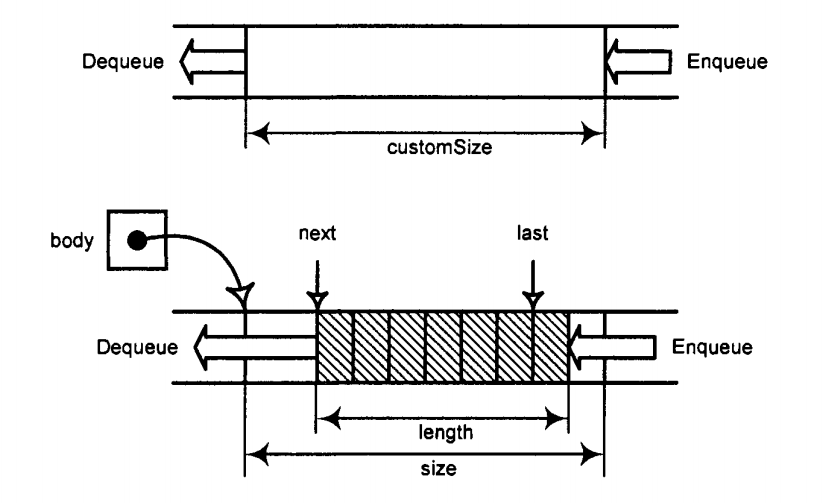
\includegraphics[scale=0.5]{images/lec05-pic01.png}
\end{figure}
\end{frame}
  
\begin{frame}{Функции - не члены класса, улучшающие инкапсуляцию}
\begin{figure}[h]
\centering
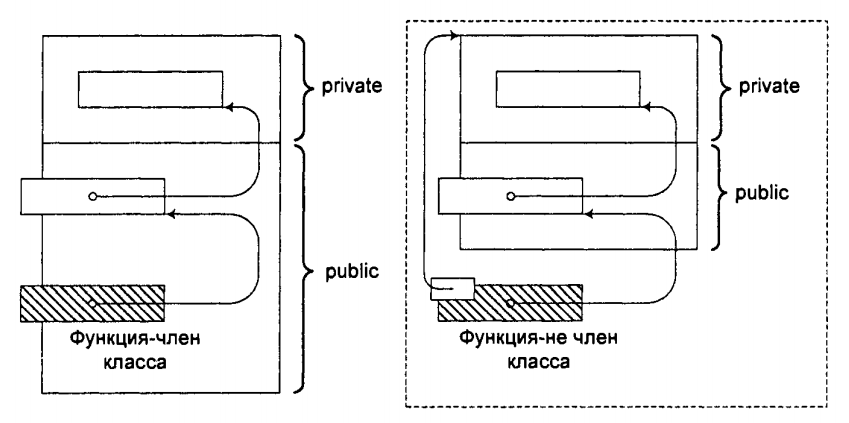
\includegraphics[scale=0.5]{images/lec05-pic02.png}
\end{figure}
\end{frame}

\begin{frame}{Инициализация объектов}
Инициализация с использованием специальной функции:
\begin{figure}[h]
\centering
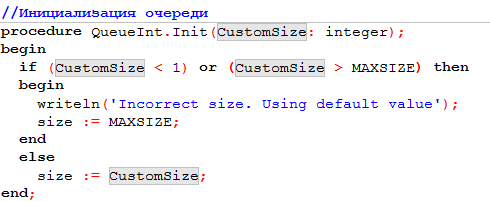
\includegraphics[scale=0.75]{images/lec05-pic03.png}
\end{figure}
\begin{itemize}
\item нигде в объявлении типа не указано, что объект должен быть проинициализирован;
\item некоторые объекты могут не нуждаться в инициализации, а для некоторых инициализация должна быть обязательной. 
\end{itemize}
\end{frame}

\begin{frame}{Конструкторы}
\begin{block}{Конструктор}
метод класса, основное назначение которого состоит в инициализации объекта
\end{block}

\begin{figure}[h]
\centering
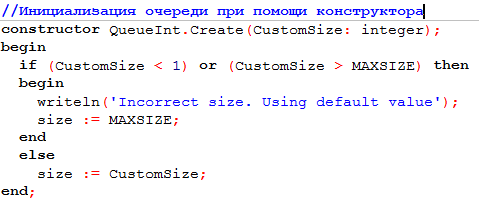
\includegraphics[scale=0.6]{images/lec05-pic04.png}
\end{figure}
\begin{itemize}
\item рекомендованное имя конструктора - Create;
\item конструктор вызывается всегда при создании объекта. 
\end{itemize}
\end{frame}

\begin{frame}{Конструкторы}
\begin{figure}[h]
\centering
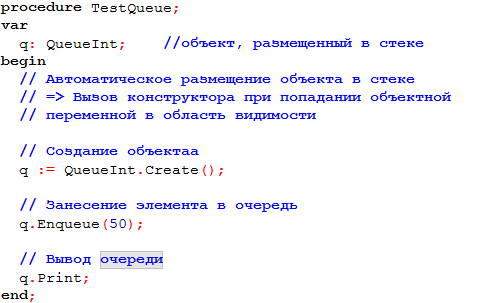
\includegraphics[scale=0.6]{images/lec05-pic05.png}
\end{figure}
\end{frame}

\subsection{Спецификация и реализация класса}

\begin{frame}
\begin{block}{Спецификация класса}
метод класса, основное назначение которого состоит в инициализации объекта
\end{block}
Спецификация:
\begin{itemize}
\item содержит информацию, достаточную для корректного использования класса. 
\item для разработчика класса должна содержать объявления всех членов класса. 
\item для пользователя должна содержать, по крайней мере, объявления открытых и защищенных членов класса. 
\end{itemize}
\end{frame}

\begin{frame}
\begin{figure}[h]
\centering
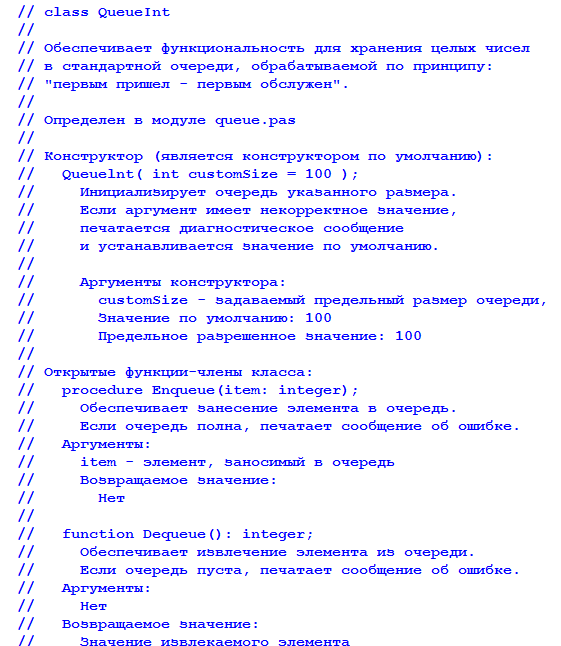
\includegraphics[scale=0.5]{images/lec05-pic06.png}
\end{figure}
\end{frame}

\begin{frame}{Обработка индексов при работе с массивом Queuelnt}
\begin{figure}[h]
\centering
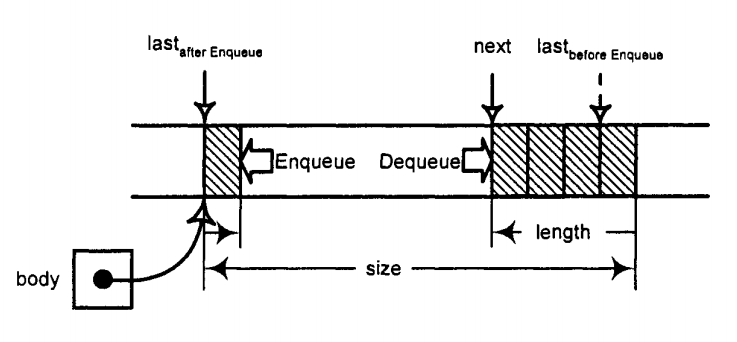
\includegraphics[scale=0.5]{images/lec05-pic07.png}
\end{figure}
\end{frame}

\begin{frame}
Недостатки приведенной реализации:
\begin{enumerate}
\item В ходе работы методов класса Queuelnt происходит печать на консоль. Это
ограничивает область применения класса только консольными приложениями.
\item Методы класса реализованы таким образом, что в случае возникновения
ошибок производится печать информации об ошибке на консоль, что может не вписываться в организацию клиентского кода.
\item Встроенная обработка ошибок работы с очередью не позволяет пользователю класса реализовать свой обработчик ошибок с учетом инфраструктуры клиентского приложения.
\item В случае, если очередь пуста, функция Dequeue() возвращает фиктивное значение, которое вполне может совпадать с одним из элементов очереди. Это может быть источником ошибок при использовании очереди.
\item Спроектированный класс позволяет хранить в очереди только целые данные. 
\end{enumerate}
\end{frame}

\section{Конструкторы и деструкторы}
\subsection{Перегрузка конструкторов}
\begin{frame}{Пример. Рациональные числа}
Класс может иметь несколько конструкторов с различными списками параметров. 
Это позволяет иметь несколько вариантов инициализации объекта.
\begin{figure}[h]
\centering
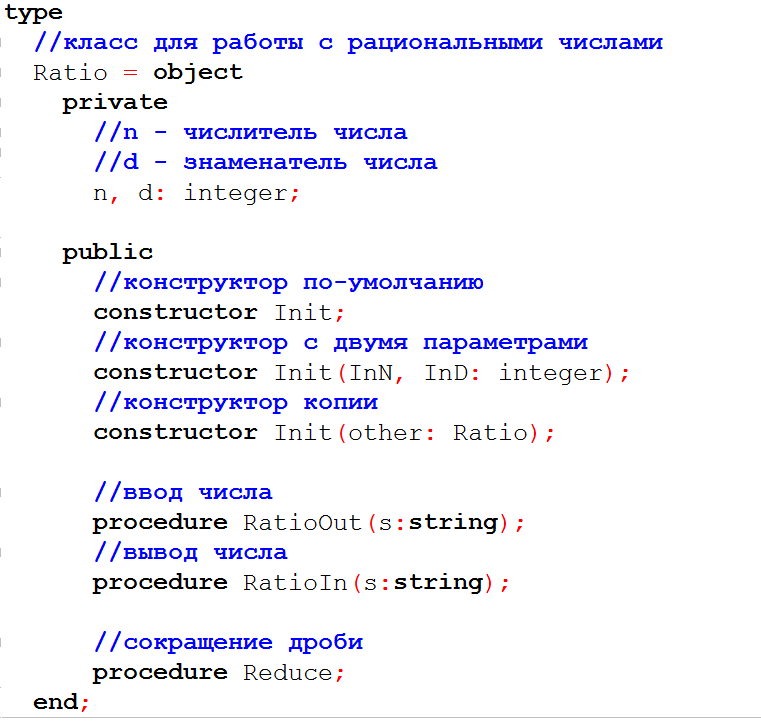
\includegraphics[scale=0.3]{images/lec05-pic08.png}
\end{figure}
\end{frame}

\subsection{Права доступа в связи с конструкторами}
\begin{frame}{Права доступа в связи с конструкторами}
Конструктор может быть объявлен с разным спецификатором доступа.
\begin{itemize}
\item Помещение конструктора в защищенную секцию делает возможным обращение к нему только в инициализаторе производного класса. 
\item Объявление закрытого конструктора запрещает инициализацию объекта определенным образом. 
\item Если класс не имеет ни одного открытого конструктора, объекты такого класса создавать нельзя. Это означает, что данный класс можно использовать только в качестве базового для других классов.
\end{itemize}
\end{frame}

\subsection{Конструкторы как преобразования типов}
\begin{frame}{Конструкторы как преобразования типов}
Конструктор, имеющий один аргумент, задает преобразование типа, то есть определяет правило преобразования типа аргумента конструктора в тип объекта.
\begin{figure}[h]
\centering
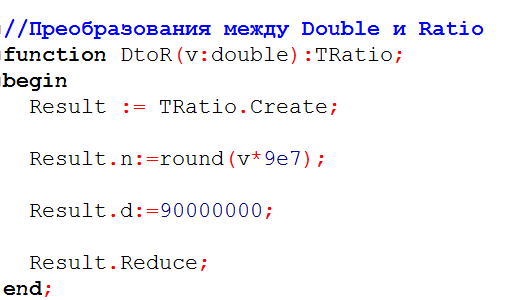
\includegraphics[scale=0.4]{images/lec05-pic09.png}
\end{figure}
\begin{figure}[h]
\centering
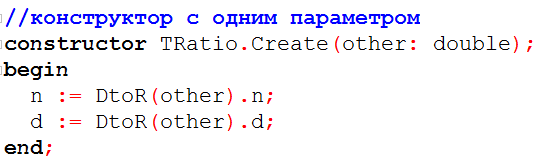
\includegraphics[scale=0.4]{images/lec05-pic10.png}
\end{figure}
\end{frame}

\begin{frame}{Конструкторы как преобразования типов}
\begin{figure}[h]
\centering
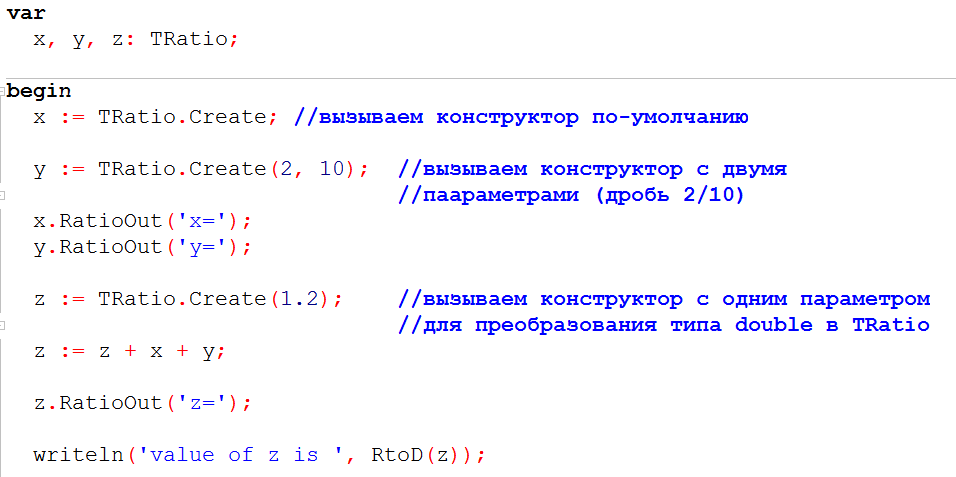
\includegraphics[scale=0.4]{images/lec05-pic11.png}
\end{figure}
\end{frame}

\subsection{Деструкторы}
\begin{frame}
\begin{block}{Деструктор}
специальный метод класса, обеспечивающий корректное разрушение среды, в которой функционирует объект.
\end{block}
\begin{itemize}
\item Иногда создание объекта предполагает помимо прочего захват каких-либо ресурсов (например, резервирование динамической памяти).
\item Для таких классов необходимо наличие метода, который будет гарантированно вызываться по окончании использования объекта.
\end{itemize}
В подавляющем большинстве случаев деструкторы вызываются неявно.
\begin{figure}[h]
\centering
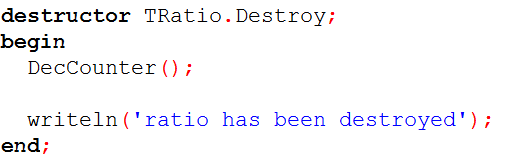
\includegraphics[scale=0.4]{images/lec05-pic12.png}
\end{figure}
\end{frame}

\section{Статические данные}
\begin{frame}
\begin{block}{Статическими члены класса}
переменных-члены класса, которые, являясь элементами класса, не являются элементами объекта, или, иными словами, являются общими для всех объектов данного класса.
\end{block}
\begin{figure}[h]
\centering
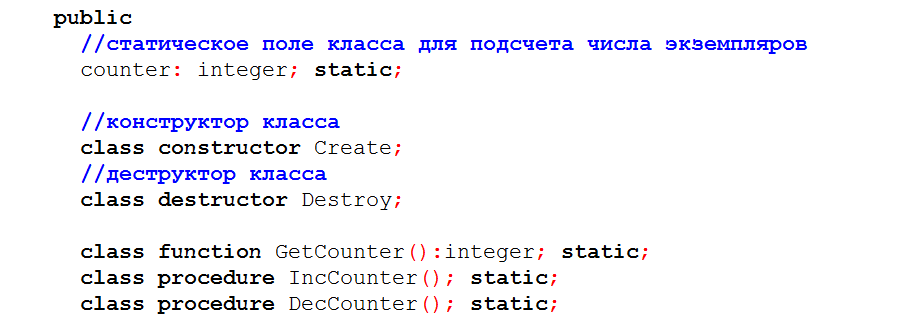
\includegraphics[scale=0.4]{images/lec05-pic13.png}
\end{figure}
Статические члены класса позволяют, с одной стороны, обеспечить требуемую в подобных случаях независимость от состояния и поведения отдельного объекта, с другой стороны — обеспечить их существование в области видимости класса.
\end{frame}

\begin{frame}
\begin{itemize}
\item К статическим членам класса можно обращаться без указания имени объекта.
\item В качестве квалификатора используется имя класса, который и образует область видимости статических данных.
\item Cтатические функции не могут обращаться к нестатическим членам класса.
\end{itemize}
\begin{figure}[h]
\centering
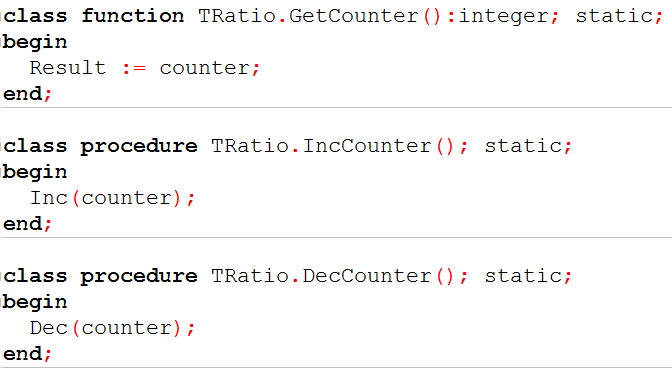
\includegraphics[scale=0.4]{images/lec05-pic14.png}
\end{figure}
\end{frame}

\begin{frame}{Статические конструктор и деструктор}
\begin{figure}[h]
\centering
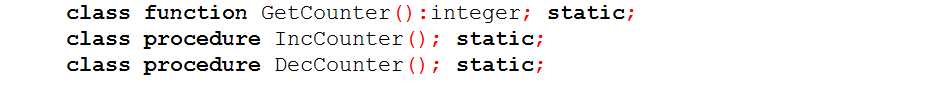
\includegraphics[scale=0.5]{images/lec05-pic15.png}
\end{figure}
\begin{itemize}
\item может сущестовать только один конструктор класса (статический конструктор) без параметров.
\item может сущестовать только один деструктор класса (статический деструктор) без параметров.
\item статические конструктор и деструктор вызываются только неявно.
\item порядок вызова конструкторов и деструкторов не определен.
\end{itemize}
\end{frame}

%\subsection{Неявный параметр self}
%\section{Перегруженные функции и операции-члены класса}
%\subsection{Перегрузка методов}
%\subsection{Перегрузка арифметических операций}
%\section{Копирование объектов класса}

\end{document}
